    \begin{figure}[h]
        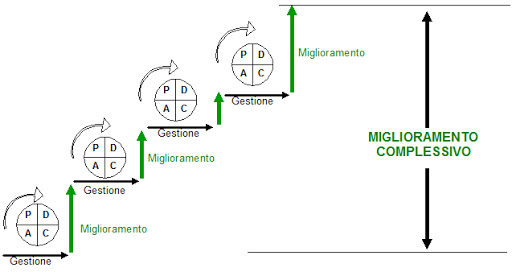
\includegraphics[width=9cm]{src/CicloDeming/img/ciclodeming.jpg}
        \centering
        \caption{Ciclo di Deming o PDCA}
    \end{figure}
	Ogni processo deve essere organizzato basandosi sul principio del miglioramento continuo (o \glo{ciclo di Deming}):
	\begin{itemize}
		\item \textbf{Plan (pianificare):} viene definito un piano che basandosi sulla definizione di problemi e obiettivi pianifica compiti, assegna responsabilità, studia il caso, analizza le cause della criticità e definisce azioni correttive;
		\item \textbf{Do (eseguire):} vengono implementate le attività secondo le linee definite durante la fase Plan;
		\item \textbf{Check (valutare):} viene verificato l’esito delle azioni di miglioramento rispetto alle attese;
		\item \textbf{Act (agire):} vengono applicate le correzioni necessarie per colmare le carenze rilevate e vengono standardizzate le attività correttamente eseguite.
	\end{itemize}